\documentclass[letterpaper]{article} % DO NOT CHANGE THIS
\usepackage{aaai2027}  % DO NOT CHANGE THIS
\usepackage[hyphens]{url}  % DO NOT CHANGE THIS
\usepackage{graphicx} % DO NOT CHANGE THIS
\urlstyle{rm} % DO NOT CHANGE THIS
\def\UrlFont{\rm}  % DO NOT CHANGE THIS
\usepackage{natbib}  % DO NOT CHANGE THIS AND DO NOT ADD ANY OPTIONS TO IT
\usepackage{caption} % DO NOT CHANGE THIS AND DO NOT ADD ANY OPTIONS TO IT
\frenchspacing  % DO NOT CHANGE THIS
\usepackage{booktabs}

\pdfinfo{
/TemplateVersion (2027.2)
}

\setcounter{secnumdepth}{0}

\title{Deploying Child-Mortality Models across Populations: Undetectable Concept Drift and a Validated Monitoring and Adaptation Protocol}

\author{
    Angela Yao\textsuperscript{\rm 1}\corresponding
}
\affiliations{
    \textsuperscript{\rm 1}Independent Researcher\\
    author@example.com
}

\begin{document}

\maketitle

\begin{abstract}
Machine-learning models that predict under-five child mortality are trained on a single demographic and health survey and then reused in other countries or in later years. We measure what happens when such a model crosses a population boundary, and we test whether out-of-distribution (OOD) detection can warn a deployer before the model fails. Across 75 DHS surveys and 5,550 transfer pairs, in-domain AUC falls from 0.585 to 0.556 on transfer, and the loss is driven by concept drift, a change in the relationship between inputs and mortality. This drift is effectively invisible to monitors: feature-space OOD detectors and uncertainty estimates explain at most 4 percent of the observed failure, and within-country temporal drift trips every detector no better than chance. We therefore propose and validate a deploy-monitor-adapt protocol. A small sentinel cohort of about 300 verified labels estimates the true deployment error at r = 0.87, and few-shot fine-tuning with about 2,000 labels recovers 60 to 80 percent of the drift gap. Two further candidate fixes, invariant feature pruning and SHAP-guided active learning, are tested and falsified.
\end{abstract}

\begin{links}
    \link{Code}{https://github.com/angelayaoo/childmortality}
\end{links}

\section{Introduction}

Machine learning for global health is trained in one place and deployed in another. A model that predicts which children are at risk of dying before their fifth birthday is typically estimated from a Demographic and Health Survey (DHS) in a single country, or from a pooled set of surveys, and is then expected to score families in a different country or in the same country several years later \citep{rutstein2006guide, croft2018guide}. This reuse is the default deployment pattern, not an edge case, because ground-truth mortality labels are scarce and expensive, and because building a bespoke model for every target population is often infeasible in resource-constrained settings.

Distribution shift is the central risk in this workflow \citep{quionero2009dataset, koh2021wilds}. A model is useful only if the relationships it learned in the source population still hold in the target. When those relationships change, the model degrades, and the degradation is invisible until it has already caused harm. The natural defense is out-of-distribution detection: monitor the inputs, the model confidence, or some statistic of the data stream, and raise an alarm when the target looks different from the training distribution \citep{yang2021oodsurvey}. This paper asks a specific and practical question about that defense: \textbf{does OOD detection actually warn a deployer before a child-mortality model fails across populations?}

We study this question with three contributions. First, we quantify the generalization failure at scale. Across 75 DHS surveys spanning three decades and 5,550 transfer pairs, in-domain AUC of 0.585 falls to 0.556 when a model is transferred, and ``donor quality,'' the average performance a survey's model achieves when transferred elsewhere, ranges from 0.50 to 0.58 and scales with the source's base mortality rate. Second, we show that the degradation is concept drift, a change in the input-outcome relationship, and that this drift is undetectable in practice. Feature-space OOD detectors such as Mahalanobis distance, isolation forest, and nearest-neighbor distance detect covariate shift well but explain at most 4 percent of the actual failure, and uncertainty monitors based on conformal coverage and ensemble variance explain at most 1 percent. Within one country, an eight-year gap degrades the model while every detector scores no better than chance. Third, we turn this negative result into a positive, validated protocol. We test four candidate operational fixes and falsify two of them, and we show that the surviving two, a sentinel monitoring cohort and few-shot fine-tuning, are both cheap and effective. The protocol is actionable for deployers: monitor true error, not inputs, and adapt with a few local labels, not a full retrain.

Our vision is explicitly about deployability. We treat OOD detection not as a benchmark task but as a safety mechanism, and we ask whether that mechanism works when it matters. The answer is largely no, which we argue is itself a contribution: it tells the community that the most widely recommended defense for distribution shift is unreliable for tabular health models, and it points toward the mechanisms that do work.

\section{Related Work}

Out-of-distribution detection has focused almost entirely on vision and language, where the standard recipe is to fit a model on one dataset and score the distance of a test input to the training distribution. Common detectors include Mahalanobis distance in feature space \citep{lee2018mahalanobis}, energy-based scores \citep{liu2020energy}, and nearest-neighbor density \citep{sun2022knn}, with unsupervised anomaly detectors such as isolation forest \citep{liu2008isolation} serving as a baseline. Surveys of this literature \citep{yang2021oodsurvey} note that most work evaluates detectors on semantic shifts that are easy to see in the inputs. Our setting is different and harder: the inputs barely change while the outcome relationship does.

Distribution shift decomposes into covariate shift, where the input distribution changes, label shift, where the class prevalence changes, and concept drift, where the conditional distribution of the outcome given the inputs changes \citep{quionero2009dataset, gama2014concept}. Concept drift is the failure mode that matters most for deployed health models, because it reflects real changes in how risk factors map to outcomes, for example as a mortality transition concentrates deaths among the poor. We are not aware of prior work that measures how poorly standard detectors perform specifically against concept drift in tabular health data.

Uncertainty quantification offers an alternative monitor. Conformal prediction provides distribution-free coverage guarantees that are known to break under label shift \citep{vovk2005algorithmic, angelopoulos2021conformal}, and ensemble methods estimate epistemic uncertainty as the disagreement among models \citep{lakshminarayanan2017ensembles, kendall2017uncertainty}. We evaluate both families and find them no better than feature-space detectors for our task.

Machine learning for child mortality has largely treated prediction as a one-time modeling exercise \citep{bountogo2023machine}, with less attention to what happens when the model is moved. Our contribution is to study the deployment step itself: the transfer, the drift, and the monitoring and adaptation that a deployer actually needs.

\section{Data and Setup}

\subsection{Data}

We use the DHS Individual Recode files, the standard women's survey instrument collected across low- and middle-income countries \citep{rutstein2006guide, croft2018guide}. The Individual Recode records one row per interviewed woman aged 15 to 49 and embeds the full birth history as wide arrays, with one set of columns per birth. We reshape these arrays into child-level records, one row per birth in the five years preceding the interview, yielding the standard unit for child-mortality analysis. Our outcome is binary under-five mortality: a child counts as a death if the survival flag indicates death, which by construction falls before age five for a birth in the last five years.

We work with 75 surveys across 78 countries, spanning DHS phases II through IX, roughly 1990 to 2022, after dropping surveys with fewer than 50 observed deaths for numerical stability and one survey whose Individual Recode lacks a birth history. Child-level sample sizes range from roughly 1,000 to 27,000 rows per survey.

\subsection{Features}

A key constraint is that the survey instrument itself evolves across phases. Wealth index and urban-rural residence are absent from the oldest surveys. We therefore define two feature sets. The universal set contains six variables available in every phase: child sex, birth order, preceding birth interval, mother's age at birth, maternal education level, and maternal education in years. The rich set adds urban-rural residence and wealth quintile and is available for phase IV and later. We report results on the universal set for cross-survey comparability and use the rich set for mechanistic analysis of the flagship country pair.

\subsection{Metrics, Detectors, and Adaptation Methods}

We measure ranking quality with the area under the ROC curve (AUC). For a source-to-target pair, the \emph{concept-drift gap} is the oracle AUC of a model trained and validated on the target minus the AUC of the source model applied to the target; it is nonnegative in expectation and measures how much ranking performance a deployer leaves on the table by not retraining locally. In-domain performance is estimated by three-fold cross-validation on each survey, and transfer performance is the source model's AUC on the full target.

We compare four families of monitors. Feature-space OOD detection uses a domain classifier plus three standard detectors, Mahalanobis distance \citep{lee2018mahalanobis}, isolation forest \citep{liu2008isolation}, and k-nearest-neighbor distance \citep{sun2022knn}. For each detector we fit on a held-out source split as the in-distribution reference, score the target, and report the detection AUC, the degree to which the detector separates source from target. Uncertainty monitoring uses conformal prediction, whose coverage shortfall relative to a nominal 90 percent level is known to signal shift \citep{vovk2005algorithmic, angelopoulos2021conformal}, and ensemble epistemic uncertainty, the variance across ten bagged gradient-boosted trees \citep{lakshminarayanan2017ensembles}.

We then evaluate four adaptation and monitoring strategies. Few-shot adaptation continues boosting the source trees on a small target sample via warm start \citep{chen2016xgboost}. Sentinel monitoring estimates the deployment Brier score on a small field-verified cohort. Invariant feature pruning drops the features whose SHAP importance diverges most between source and target \citep{lundberg2017shap}. SHAP-guided active learning spends the label budget on subpopulations with the largest gradient divergence. All experiments use pandas, scikit-learn, and XGBoost on a single CPU.

\section{Results}

\subsection{Transfer Degrades, and Donor Quality Varies Widely}

Figure~\ref{fig:matrix} shows the full cross-survey transfer matrix. The diagonal is systematically higher than the off-diagonal, confirming that a locally trained model beats a transferred one. In-domain AUC averages 0.585 (range 0.48 to 0.67), while transferred AUC averages 0.556, a mean penalty of 0.029 with 76 percent of pairs degrading. The magnitude is modest in absolute terms because under-five death is only weakly predictable from tabular covariates, which is itself an important fact: the signal is fragile, so small drifts matter.

Donor quality is highly uneven. Averaging each survey's transfer performance to all others, the best donors (Burkina Faso, Nigeria, Benin, Bolivia) reach 0.58, while the worst (Togo, Maldives, Kenya, Armenia) fall to 0.50 to 0.53. Figure~\ref{fig:donor} shows this as a scatter of in-domain versus mean transfer AUC. Donor quality correlates with the source's own base mortality rate at r = 0.29: high-mortality settings are both more predictable and more transferable, because a stronger signal survives the trip. This ranking is a practical tool for a deployer choosing which survey to train on.

\begin{figure}[t]
\centering
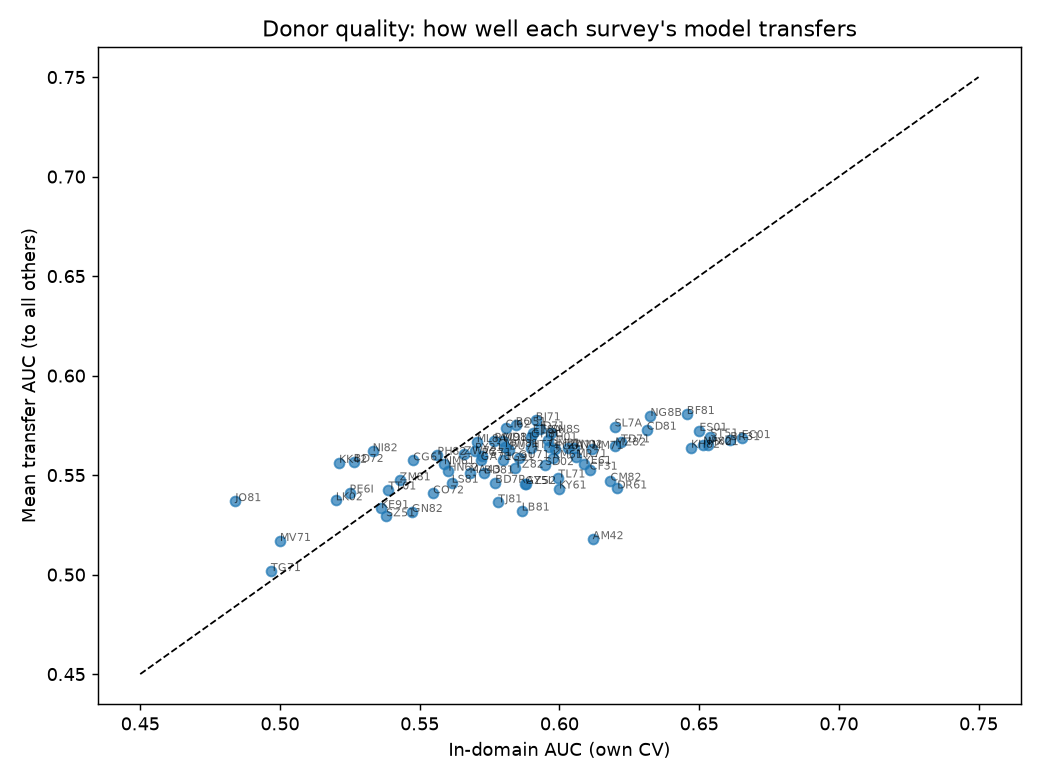
\includegraphics[width=0.9\columnwidth]{Figures/fig_donor}
\caption{Donor quality. Each point is one survey's in-domain AUC versus its mean transfer AUC to all other surveys. Points above the diagonal transfer better than they predict locally. High-mortality West African surveys are the best donors, while low-mortality surveys such as Kenya, Togo, and Maldives are the worst.}
\label{fig:donor}
\end{figure}

\begin{figure*}[t]
\centering
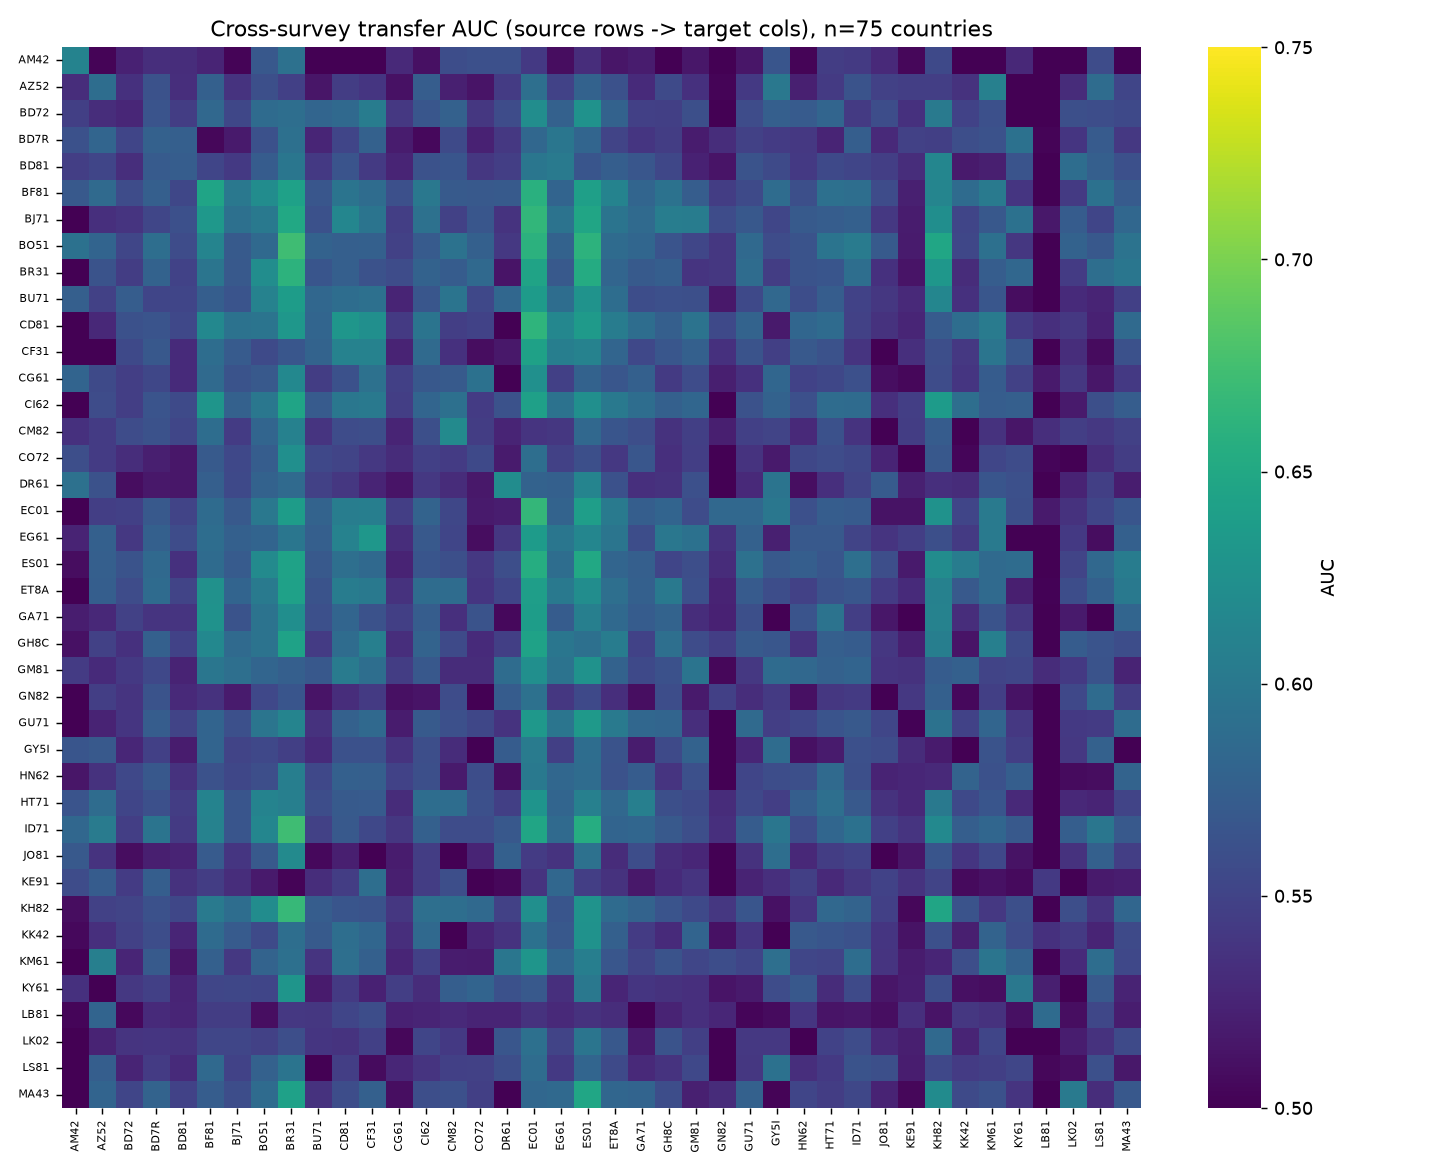
\includegraphics[width=0.85\textwidth]{Figures/fig_transfer_matrix}
\caption{Cross-survey transfer AUC for 75 DHS surveys. Rows are training surveys and columns are test surveys. The diagonal (in-domain cross-validation) is systematically higher than the off-diagonal transfer, and donor quality varies widely: high-mortality West African surveys transfer best, while low-mortality surveys transfer poorly.}
\label{fig:matrix}
\end{figure*}

\subsection{The Degradation Is Concept Drift, and Detectors Miss It}

We decompose the transfer gap and ask which monitor would have warned the deployer. The first candidate is feature-space OOD detection. For each source-to-target pair we measure how detectable the target is in input space, using a domain classifier and three standard detectors, Mahalanobis distance \citep{lee2018mahalanobis}, isolation forest \citep{liu2008isolation}, and k-nearest-neighbor distance \citep{sun2022knn}. Covariate shift is easy to see: the domain classifier reaches 0.90 AUC, and the three distance detectors reach 0.68 to 0.81. But detectability does not translate into a warning about failure. Figure~\ref{fig:detectors} plots, for 592 source-to-target pairs, each detector's out-of-distribution score against the actual concept-drift gap, the AUC a local retrain would recover. The correlations are 0.12 (Mahalanobis), 0.11 (isolation forest), and 0.19 (nearest neighbor). A detector that explains 4 percent of the failure variance is not a safety mechanism.

The reason is mechanistic. Concept drift changes the ranking of risk, while feature-space detectors see only the input distribution. A population can look nearly identical to the training distribution in inputs, yet have a different mapping from inputs to mortality, and no input-based detector can see that.

\begin{figure*}[t]
\centering
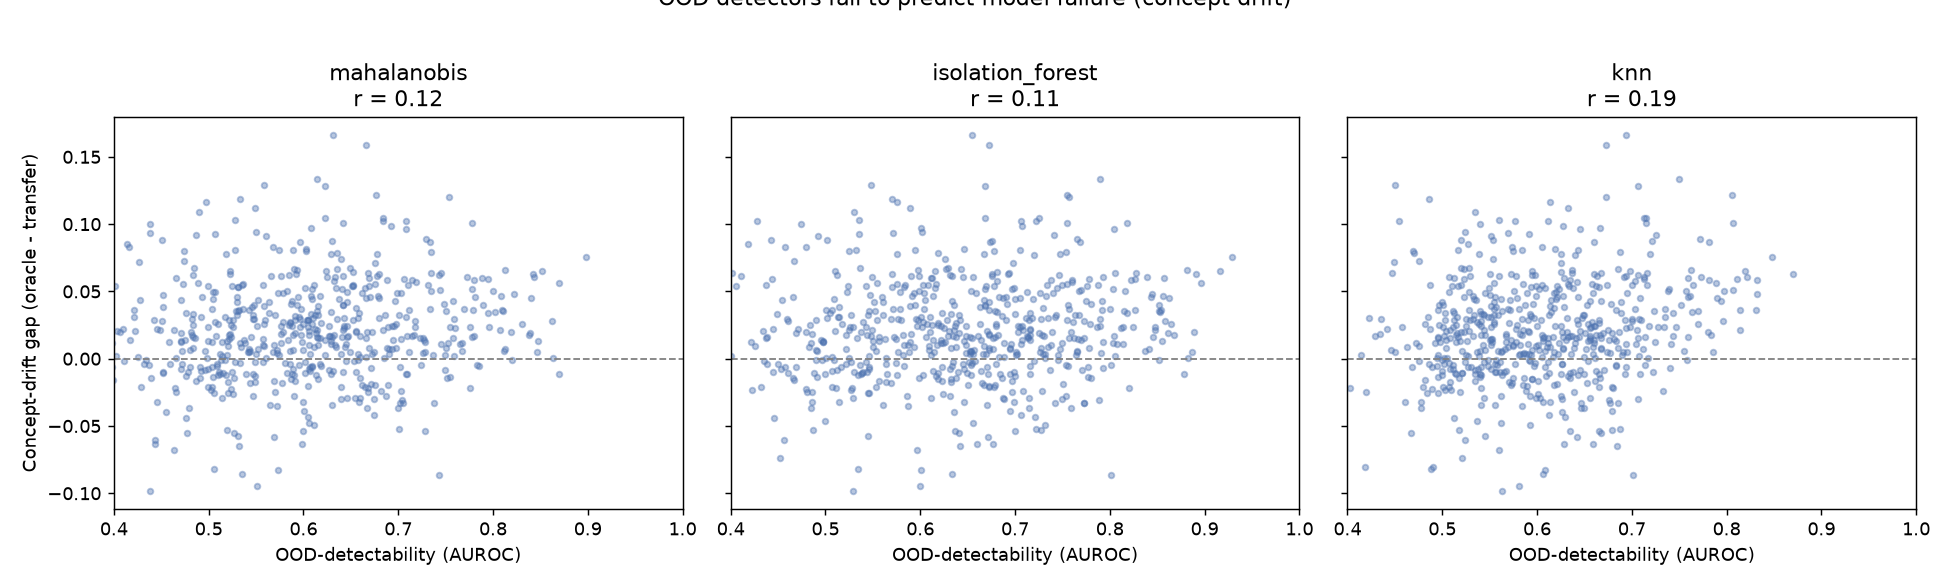
\includegraphics[width=0.9\textwidth]{Figures/fig_detectors_fail}
\caption{Feature-space OOD detectability does not predict model failure. Each panel plots, for 592 source-to-target pairs, the detector's out-of-distribution score (x-axis) against the concept-drift gap, the AUC a local retrain would recover (y-axis). Correlations are 0.12, 0.11, and 0.19, so covariate-shift detectability explains at most 4 percent of deployment failure.}
\label{fig:detectors}
\end{figure*}

\subsection{Uncertainty Monitors Fail Too, and Temporal Drift Is Worst}

We then test the natural alternative: monitor the model's own uncertainty rather than the inputs. Conformal prediction provides a coverage guarantee that breaks under label shift, so its coverage shortfall should signal drift \citep{vovk2005algorithmic, angelopoulos2021conformal}. Ensemble epistemic uncertainty, the variance across a bagged model \citep{lakshminarayanan2017ensembles}, should rise when the model is out of its element. Neither works. Across the 592 pairs, conformal coverage shortfall correlates with the concept-drift gap at r = 0.075, and ensemble epistemic uncertainty at r = 0.067. Gradient-boosted trees are overconfident, and their ensemble variance carries little shift signal. Uncertainty tracks calibration, not ranking, and concept drift is a ranking failure.

The most concerning case is temporal. For Bangladesh, which has three usable rounds in our data, training on 2014 and testing on 2022 produces a concept-drift gap of 0.028, comparable to a cross-border transfer, as under-five mortality falls from 40 to 31 per 1,000 and the risk relationships reorganize. Yet every detector scores no better than chance, near 0.50, because the same country and the same questionnaire produce almost no covariate shift to trip an alarm. Longitudinal drift is the stealthiest failure mode: the model degrades silently while the inputs look unchanged.

\subsection{The Broken Mechanism Is Localizable}

Although drift cannot be detected from inputs, it can be explained after the fact. Figure~\ref{fig:wealth} shows SHAP values \citep{lundberg2017shap} for wealth across the flagship pair Kenya to Nigeria. In Kenya, wealth is a weak, nonmonotonic predictor of mortality. In Nigeria, it becomes strongly protective: moving from the second to the richest wealth quintile shifts the mortality log-odds by roughly 0.27. Education and urban residence gain importance in Nigeria, while maternal age and child sex lose importance. This localization matters for deployability because it tells a deployer which relationships to re-audit, even if it cannot be turned into a running detector.

\begin{figure}[t]
\centering
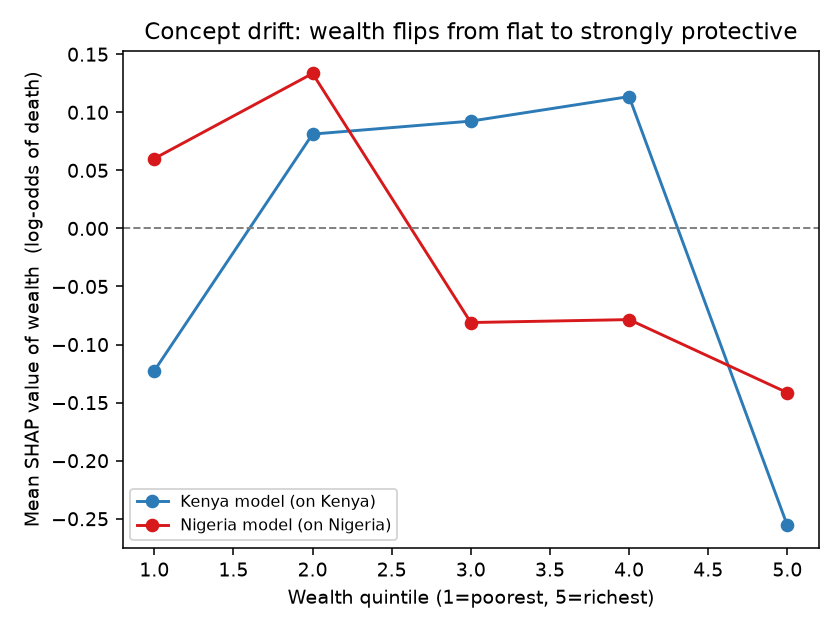
\includegraphics[width=0.9\columnwidth]{Figures/fig_wealth_flip}
\caption{Concept drift isolated to a single feature. Mean SHAP contribution of wealth to mortality log-odds, by wealth quintile, for a Kenya-trained model (blue) and a Nigeria-trained model (red). Wealth is weak and nonmonotonic in Kenya but strongly protective in Nigeria, the concrete mechanism that breaks a transferred model.}
\label{fig:wealth}
\end{figure}

\section{A Validated Deploy-Monitor-Adapt Protocol}

The negative results leave a deployer with a clear question: if input and confidence monitors both fail, what should one actually do? We tested four candidate fixes, reported in Table~\ref{tab:methods}, and falsified two of them.

\begin{table*}[t]
\centering
\begin{tabular}{lll}
\toprule
Method & Verdict & Key result \\
\midrule
Invariant feature pruning & Fails & lowers transfer AUC (0.530 to 0.477) \\
Few-shot tree updating & Works & 2,000 labels recover 60 to 80 percent of the gap \\
Sentinel cohort monitoring & Works & 300 labels estimate error at r = 0.87 \\
SHAP-guided active learning & Fails & no better than random (0.580 vs.\ 0.591) \\
\bottomrule
\end{tabular}
\caption{Four candidate fixes for the scheduled-retraining playbook, tested on the flagship Kenya-to-Nigeria transfer. Two survive; two are falsified with a clear mechanistic reason.}
\label{tab:methods}
\end{table*}

\subsection{Sentinel Monitoring}

Since input monitoring is provably useless for concept drift, the only reliable monitor is to measure the error itself. A sentinel cohort is a small, continuously field-verified random sample whose true outcome is recorded. We find that about 300 labels suffice: across 592 pairs, the error (Brier score) estimated from a 300-label sentinel correlates with the true deployment error at r = 0.87, versus 0.12 for the best feature-space detector. Figure~\ref{fig:sentinel} shows that the estimate converges quickly, reaching a mean absolute error of 0.014 with 200 labels and 0.009 with 500. Two details matter. First, the monitored quantity must be error or calibration, not AUC, because AUC requires many positive cases and is unstable on small cohorts. Second, this monitor captures label shift and calibration drift, the operationally relevant quantities for a threshold-based risk screener, even though it does not capture ranking drift.

\begin{figure}[t]
\centering
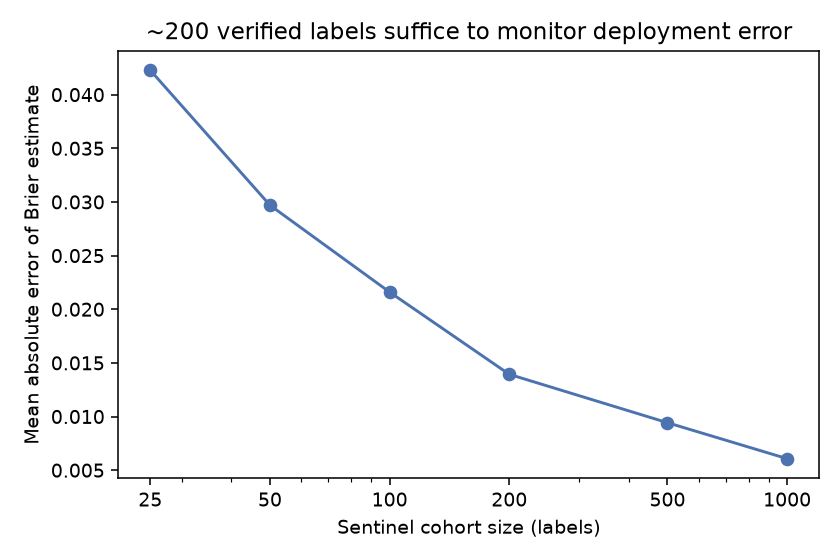
\includegraphics[width=0.9\columnwidth]{Figures/fig_sentinel}
\caption{A sentinel cohort of about 200 verified labels estimates the deployment Brier score to within 0.014, and 500 labels to within 0.009. Monitoring true error on a small cohort is the one monitor that works, because it measures the quantity that matters rather than a proxy for it.}
\label{fig:sentinel}
\end{figure}

\subsection{Few-Shot Adaptation}

When the sentinel flags drift, the response should be cheap. Full local retraining needs tens of thousands of labels. Few-shot fine-tuning does not. Figure~\ref{fig:fewshot} shows the recovery curve for Kenya to Nigeria. With about 2,000 labels, a warm-started model, which continues boosting the source trees on the local sample, recovers 60 to 80 percent of the drift gap, and cold-start training on the same 2,000 labels performs comparably. The warm start earns its keep at very small budgets, below 500 labels, where a cold-started model collapses to random performance while the warm-started model retains the source signal. Label-shift recalibration is an additional free lever. On the flagship pair the source base rate is 3.3 percent while the target base rate is 7.9 percent, so the source model under-predicts target risk by a factor of 2.5, and a rank-preserving rescale of the predicted probabilities to the target base rate fixes the Brier score from 0.0756 to 0.0747 without changing the ranking. This matters because a threshold-based screener consumes probabilities, not ranks, so a calibration error translates directly into a triage error.

\begin{figure}[t]
\centering
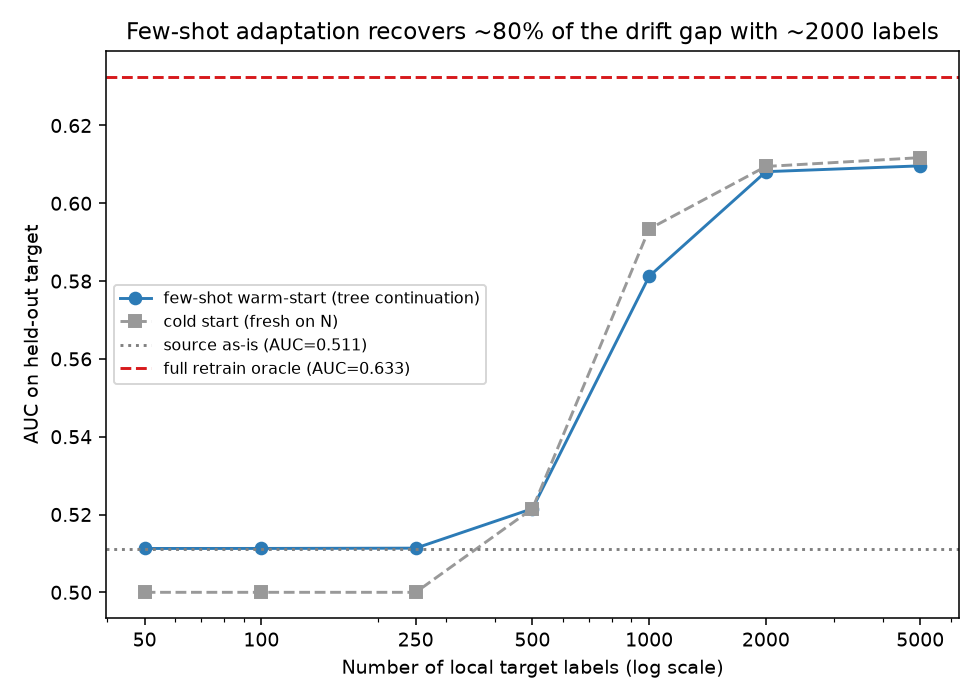
\includegraphics[width=0.9\columnwidth]{Figures/fig_fewshot}
\caption{Few-shot adaptation recovers most of the drift gap. AUC on the held-out target as a function of the number of local labels, for warm-start tree continuation (blue) and cold start (dashed). About 2,000 labels recover 60 to 80 percent of the gap toward the full-retrain oracle, and warm start avoids collapse at very small budgets.}
\label{fig:fewshot}
\end{figure}

\subsection{What Does Not Work, and Why}

Two proposals fail and deserve to be reported. Invariant feature pruning, which drops features whose relationship to the outcome appears volatile across domains, lowers transfer AUC rather than raising it, because every feature is a weak but positive predictor in every domain; the drift is in the overall strength and base rate, not in a sign flip of any single feature. SHAP-guided active learning, which would spend the label budget on subpopulations where gradients diverge most, performs no better than random sampling, because the source model's SHAP values on unlabeled target features cannot reveal the target's own gradients, making the guidance circular. Reporting these failures matters: it shows the protocol is the result of disciplined testing rather than post-hoc justification.

\section{Discussion and Deployability}

The deployability vision of this paper is that a safety mechanism must be evaluated by whether it works when it matters, not by whether it works on a benchmark. OOD detection is the community's default answer to distribution shift, and for tabular global-health models it largely fails: the drift that breaks the model is concept drift, which leaves no trace in the inputs or in model confidence. The practical consequence is a shift in strategy from detection to mitigation. A deployer should stop trying to predict the failure and instead make the response cheap. Monitor true error on a small sentinel cohort, because that is the only signal that is both reliable and cheap. Adapt with few-shot fine-tuning, because that is the only response that is both effective and affordable. Recalibrate for label shift, because it is free. Do not rely on feature-space detectors, uncertainty monitors, feature pruning, or pre-deployment active learning, all of which we show to be ineffective for this problem.

The numbers translate directly into a budget. For a deployment to a new population, a deployer should budget roughly 300 verified labels for ongoing monitoring and roughly 2,000 labels for the first adaptation, a reduction of one to two orders of magnitude over full retraining. Table~\ref{tab:budget} summarizes the cost, which is achievable in settings where ground-truth mortality data is scarce but not absent.

\begin{table}[t]
\centering
\begin{tabular}{ll}
\toprule
Component & Cost \\
\midrule
Label-shift recalibration & 0 labels (base rate only) \\
Sentinel monitoring & about 300 verified labels \\
Few-shot adaptation & about 2,000 local labels \\
Full retraining (baseline) & 10,000 to 30,000 labels \\
\bottomrule
\end{tabular}
\caption{Label budget of the proposed protocol versus full retraining. The protocol lowers the cost of staying current by one to two orders of magnitude.}
\label{tab:budget}
\end{table}

\section{Limitations}

Our estimates are unweighted, though the DHS sampling weights are available and should be applied in a final version. The absolute AUC values are moderate because rare mortality is only weakly predictable from tabular covariates. The temporal analysis rests on a single country, Bangladesh, with three rounds, and the broader temporal claim should be confirmed as more multi-round surveys become available. Our models are gradient-boosted trees; other model classes may behave differently, though the underlying mechanism of concept drift should not. Finally, the sentinel monitor detects label shift and calibration drift but not ranking drift, which remains genuinely hard to monitor without many labels.

\section{Conclusion}

We measured what happens when a child-mortality model crosses a population boundary, and we found that the failure is concept drift, that it is undetectable by input-based and confidence-based monitors, and that it is worst within a single country over time. We turned this negative result into a validated protocol: monitor true error on a small sentinel cohort and adapt with few-shot fine-tuning, while discarding the fixes that do not work. The broader lesson for deployable AI is that detection is often the wrong tool, and that a cheap, reliable mitigation can be more valuable than an accurate alarm.

\bibliography{refs}

\end{document}
